\documentclass[a4paper,12pt]{article}
\usepackage{url,graphicx,a4wide,enumitem}
\usepackage[english]{babel}
\usepackage[utf8]{inputenc}

\parindent0pt
\parskip3pt

\renewcommand\refname{References and Notes}

\title{Criticism of Henry Mintzberg's Theses on Management}

\author{Felix Walter}

\date{October 31, 2021}
\begin{document} 
\maketitle 

\begin{abstract}
This paper was written in the context of the seminar Complex Systems and
Co-Operative Action and serves as a critical comparison of arguments in
relation to Henry Mintzberg's theses about management and the social processes
in the form of organizations.
\end{abstract}
\begin{quote}
  “I argue for a return to balance, for intuition to be allowed alongside
  analysis and recognized as a necessary process in organizations.” - Henry
  Mintzberg \cite{Mintzberg}
\end{quote}
\thispagestyle{empty}
\newpage
\tableofcontents
\newpage

\section{Introduction}

For the consideration of a system-theoretical comparison of management
theories an analysis from different points of view is to be made, which makes
it possible to point out, apart from socially available, individual knowledge
of management, a structured, practical procedure, which makes an
institutionalized application comprehensible. Furthermore, the tactical,
momentary behavior at the management level is abstracted so that it can be
conceptualized in a conceptual generalization regarding the structures of an
organization and its management and further meet a scientific reflection that
summarizes the methodology of management and generates tools of analysis.

In this paper, Henry Mintzberg's theses on management and organizations will
be critically examined with the help of concepts from management theory and
technical systems. The aim is to question Mintzberg's analogies and concepts
from a real-world implementation and to compare his view with concepts of
systems theory. Special focus is put on the development of strategies in
relation to management processes and how they are applied in an organization
according to Mintzberg. The characteristics of different forms of
organizations are compared with the concepts of a socio-technical system and
put into context. Mintzberg's theses on social structural change through
organization will finally be subjected to a critical examination.

Henry Mintzberg (*02.09.1939), a professor of economics and management at
McGill University in Canada, refers in his book \emph{Mintzberg on Management}
\cite{Mintzberg} to prevailing explanations of how an organization can
successfully achieve its goals through appropriate management by analyzing the
subject of the organizational process, the manager, in its form of execution
and highlighting society as an organizational pattern. The goal of his
consideration is to formally categorize the activities that constitute
managers in order to anticipate assumptions about successful management and,
finally, to define strategy development as a craft process. An emergent
approach by focusing on the characteristics of managers is postulated by him
to infer the success of the overall organization from the capabilities of the
manager. This approach is discussed in more detail below.

\section{Manager}

To study the characteristics of the manager, Mintzberg looks at the everyday
actions of people in management positions in different industries. He compares
various assumptions and relates them to his observations. He begins by stating
the belief that managers must be conscious, systematic planners in order to
run organizations successfully. The extent to which conscious and systematic
activity is designed is not further defined, nor is it explained why these
assumptions should hold. Through his observations, Mintzberg concludes that a
manager's actions are brief, varied, and discontinuous, and beyond that, there
are no planning activities that are manifested through an external action.

These assumptions are substantiated by Mintzberg's research in \emph{The
  Nature of Managerial Work} \cite{Mintzberg2}, Robert H. Guest \emph{Of Time
  and the Foreman} \cite{guest}, and Rosemary Stewart \emph{Managers and their
  Jobs} \cite{stewart}.  This is immediately followed by the criticism of the
"classical literature" that "managing does not produce reflective planners"
\cite[p.25]{Mintzberg}.  Mintzberg does not give any examples or details of
what "classical literature" is supposed to be, let alone what exactly it says.
According to Mintzberg, planning or goal setting cannot be actions separate
from the work process. "Managers seem to meet planning needs implicitly in the
context of daily actions, not some kind of abstract process [...]"
\cite[p.25]{Mintzberg}.  Following this, he negates the statement that
managers do not have regular duties to perform by highlighting research in
\cite{Mintzberg2} and Robert T. Davis \emph{Performance and Development of
  Field Sales Managers} \cite{davis}, which purports to prove that managers
perform a number of regular duties such as ritual, ceremony, and negotiation,
as well as processing soft information in their daily work.

No mention is made of how often managers must perform these "duties," what
planning processes might be set in motion by the "duties", or the extent to
which they measurably contribute to the success of the organization. Next, the
assumption that "managers in top positions [...] need aggregated information
[that] is best provided by a management information system" is questioned, in
which Mintzberg refers to the researches of Stewart \emph{Managers and Their
  Jobs} \cite{stewart2} and Tom Bums \emph{The Directions of Activity and
  Communication in a Departmental Executive Group} \cite{burns}, in which,
according to Mintzberg, it was found that "managers [...] very much prefer the
linguistic medium -- i.e. telephoning and face-to-face meetings"
\cite[p. 26]{Mintzberg}.  The research mentions that "managers [spend] an
average of 66 to 80 percent of their time on oral communication. The reason
for this is given in the "early warning function" of so-called "soft
information".  "Today's gossip can be tomorrow's reality"
\cite[p. 27]{Mintzberg}. It is important to note that the external sources
used are all from the 1950s.  This comment is later picked up by Ansoff
\cite{ansoff}.  Neither is this statement supported by facts, nor are figures
given as to how far "gossip" actually occurs in reality. Thus, Mintzberg
further claims that "managers [apparently do not] document [...]  what they
hear. Therefore, the strategic database of the organization lies less in the
computers than in the heads of its managers."  \cite[p. 27]{Mintzberg}.

Why Mintzberg infers low documentation of planning processes from increased
oral communication is not apparent. The connection between implicit planning
by the subject and lack of explicit presentation of decision patterns is not
explained by any evidence. Already here it becomes apparent that Mintzberg,
starting from the manager's form of description, concludes to a prescription
for successful management, which is not carried out argumentatively, but
elevated to a law by assumptions alone. Later, this logical impurity will be
described more clearly. Last, the assumption that "management [...] [is] a
science and a profession, or [...] [can] quickly develop into one"
{}\cite[p.28]{Mintzberg} shall be refuted, since "managers' programs [...]
[remain] hidden deep in their minds" \cite[p. 28]{Mintzberg}. It is more
closely indicated what Mintzberg means by "deep in the mind" by introducing
the terms "judgment" and "intuition" but not explaining them in any way. Only
the argument of "oral communication" again finds a way into the description:
"The manager is overloaded with obligations: but he cannot simply delegate his
task. Therefore he has to overwork himself and is forced to do a lot of things
superficially. Brevity, fragmentation, and oral communication characterize his
work." \cite[p. 28]{Mintzberg}. Neither evidence of commitment overload nor
the compulsion to overwork and subsequent superficiality is presented. At no
time is it apparent why Mintzberg makes these statements.

\subsection{Roles of the Manager}

He defines the manager's characteristics in terms of several roles a manager
\cite{Mintzberg} assumes, conditioned by his formal authority and status over
the organization. He has responsibility over decisions as well as over
employees and subgroups. Information is gathered and shared by the
manager. The roles are divided into three areas, which he calls interpersonal,
informational and decision-making roles, which are elaborated below.

The interpersonal roles are subdivided into representative figure, managerial
figure, and contact figure. As a representative figure, the manager must
attend ceremonies and conduct routine affairs. There is hardly any
communication that influences important decisions of the
organization. Presence in public is the decisive task here. As a leader, the
manager carries formal leadership over the organization and hires and trains
employees. The potential power enables him to make important decisions and to
instruct and motivate employees for the tasks. As a contact person, important
information is gained, which is secured and expanded by building an external
information system with influential contacts. Communication here is mostly
informal, private and verbal.

Information roles are defined as monitor, distributor, and spokesperson. As
monitor, the manager scans the environment for information and obtains it
through the network of contacts he has built. Gossip, rumors, and speculation
are part of the information-gathering process, which usually occurs in verbal
form. As a distributor, the information gained is passed on to employees who
otherwise would not have access to it or would find it difficult to
access. Going further, as a spokesperson, the manager has the task of making
speeches to external people and advocating for the needs of the
organization. He must inform and satisfy influential people who control the
organizational unit. Directors or shareholders thus receive information about
the financial condition of the organization.

Mintzberg highlights the decision-oriented roles in the four roles of
entrepreneur, crisis manager, resource allocator, and negotiator. As
entrepreneur, the manager initiates new development projects and controls and
delegates them. The department belonging to him should improve and adapt to
the changing environmental conditions. As a crisis manager, he responds to
external constraints that affect the organization. Constraints include
circumstances such as strikes, bankruptcies, or delivery problems. As a
resource allocator, the manager decides who gets what in the organization and
to what extent. Decisions are coordinated so that there are no
discontinuities. Last, as a negotiator, the manager negotiates access to
resources and important information with influential people.

The listed roles of the manager form a gestalt that, according to Mintzberg,
cannot be divided or considered separately. Every manager must pay equal
attention to all roles in order to create the necessary conditions for
successful management. It is the integration of all components that makes a
person a manager. The roles are hierarchized starting from the formal
authority, to the interpersonal, information roles and finally
decision-oriented roles in this order, thus placing the existence condition on
the respective previous roles. This gradation is not explained, nor is
evidence presented for this assumption. In the following explanations these
roles are also not mentioned again at any time or put into relation with the
assertions to the strategy development, organization or society. What function
the presentation of the roles fulfills or why Mintzberg introduces them does
not find any logical justification in his description, nor any practical
application. The form of representation is limited solely to the subjective
view of the manager and is not related to a collective management
process. This fact is later related to the definition of strategy development.

\section{Mintzberg's Model of Strategy Formation}

\subsection{The emergent strategy}

According to Mintzberg, a strategy is "plans for the future and patterns from
the past" \cite[p. 41]{Mintzberg}. The pursuit of this strategy reflects the
practice of a "realized strategy" \cite[p. 41]{Mintzberg}. The development of
a strategy is described as an emergent process that relies solely on
involvement and a sense of familiarity. Mintzberg compares strategy
development to an artistic process of creation based solely on long experience
and involvement. His assumption is therefore that organizations must pursue
emergent strategy development based solely on successful experience and
experimentation. Similar to the artist, the manager surrenders to "calculated
chaos" \cite[p. 40]{Mintzberg}.

Strategy development, according to Mintzberg, generates a logical plan through
past patterns of experience. In this process, strategies are not meant to be
made explicit, but to dwell in the "minds of managers." Moreover, he asserts
that strategies should not be formulated in both unpredictable and predictable
environmental conditions. Managers should not make assumptions about strategy
apart from their experience. Two exceptions are: The organization is newly
initiated and must make initial conceptualizations, or it is coming out of a
period of transition into a stable situation. Mintzberg exacerbates this
assumption by saying that "the long-held image of planning in the literature
distorts these processes [of strategy development] and [...] thus misleads
those organizations that rely unreservedly on planning"
\cite[p. 42]{Mintzberg}.

Developing a strategy is a process that, apart from conscious planning, refers
to stability, discovering discontinuities, knowing the industry, pattern
recognition, and the interplay between change and continuity. Using the term
"strategic learning," Mintzberg points out that "a purely planned strategy
[...] precludes [learning] once the strategy is formulated. The "emergent
strategy described earlier reinforces it" \cite[p. 45]{Mintzberg}. In doing
so, he excludes the absolute forms: "None of the approaches is very useful if
pursued in the extreme. Learning must be coupled to control."
\cite[p. 45]{Mintzberg}.

Further, Mintzberg refers to the different strategy approaches in the analogy
of the left and right hemispheres of the brain to represent the opposite forms
of rational, logical and intuitive, artistic strategy development.
Accordingly, the left brain functions in linear patterns and is fixated on
logical conclusions. On the other hand, in the right hemisphere, influences
are generally processed simultaneously and subconsciously. Especially the
perception and processing of images and sensual influences is attributed to
the right side. Mintzberg states in this comparison that managing should be
carried out to a high degree starting from the right brain hemisphere. For
example, the recognition of facial features of other persons, the correct
interpretation of voice tones or gestures or the processing of "soft
information" is crucial for the management process. Preferably, then, there is
a relational, simultaneous aggregation of information that takes place by the
manager in the subject.

According to Mintzberg, "hearsay," gossip, hallway conversations, or the like
are a decisive factor for management success. He speaks of an increased
synthesis process in which rational analysis plays a minor role. As a result,
Mintzberg says, "I therefore hypothesize that the important processes of
managing organizations depend in large part on right-brain skills."
\cite[p. 63]{Mintzberg}.

Planning, as mentioned above, should take place only under stable conditions
and, complementarily, only when innovative strategy pursuit is not necessary.
Communication of results to top management should always be verbal. In
summary, Mintzberg gives the work instruction: "Plan with the left, manage
with the right" \cite[p. 57]{Mintzberg}.

What is clear in his reflection is that he is particularly critical of the
teaching of practices of management which, according to him, "basically [have]
led modern management schools to worship the left hemisphere."
\cite[p. 68]{Mintzberg}. Mintzberg does not provide any further evidence here
outside of his aforementioned observations showing the failure of the "right
hemisphere" to emerge, nor what he means by stable environmental conditions
and innovative strategy measures.

"Some of the best-known management schools have basically become closed
systems in which professors with little interest in organizational reality
teach inexperienced students mathematical, economic, and psychological
theories as ends in themselves. In these management schools, management is
given only a small place. Our schools need a new balance, namely the best
possible balance between analysis and intuition." \cite[p. 68]{Mintzberg}.

Finally, Mintzberg refers to the "insights about consciousness"
\cite[p. 68]{Mintzberg} being suppressed by "artificial mystifying behavior".
Neither the concept of "consciousness", nor the "proper balance between
analysis and intuition" is elaborated by him. The implementation of his
hypothesis in a practical context does not receive any shape and can be
understood only as a criticism of the management schools, which is evident
only in the comparison of the concepts of analysis and intuition.

\subsection{Hemispheres of the brain}

The comparison of left and right brain hemispheres and their functions has
already been considered by Julian Jaynes in his theory of the bicameral mind
\cite{Jaynes}. Jaynes hypothesizes that the emergence of language is a
necessity for consciousness. In his theory, human development in terms of
perception is presented as the emergence of consciousness, which is not the
foundation in human existence. Consciousness is a "learned process based on
metaphorical language." Neurological studies in Jayne's presentation show
activity of the right temporal-parietal lobe during auditory hallucinations,
which corresponds to the language area of the left hemisphere. Studies of
patients whose cerebral hemispheres have been split show that they "function
as two independent persons." Bicamerals, or modern schizophrenics, perceive
hallucinations emanating from the right hemisphere as coming from outside
themselves. The right hemisphere of the brain is said to have a language
function, which people perceive as the "language of the gods." The excitation
of the right temporal lobe is therefore associated with an increased
religiosity or experience of God. The hallucinations here are often critical
in nature, such that the right hemisphere tends to "look down on the left
hemisphere."

Through various assumptions, which will not be further explained here, Jaynes
therefore postulates a developing self-awareness through an "external"
influencing factor by the right hemisphere. Mintzberg similarly names this
influencing factor in his way of looking at the nature of management by the
right hemisphere, without explaining the development of consciousness. The
intuitive, strategic learning model postulated by Mintzberg is given a
framework by this way of looking at things, which is found in a kind of "image
of God" through the organizational structure. Therefore, the objection in
\cite{seminar} that "in this process [...] strange structures [emerge] as
described in "Mintzberg on Management," where "an orientation structure is
[given] in linguistic form that the management novices [have] to follow and
adopt, while these rules are not necessarily applied by the same management
gurus who teach the novices." is understandable.

the distinction already made above between practical management at level 1,
systematic application of management experience at level 2, and its academic
study at level 3 is considered inconclusive by Jaynes' and Mintzberg's theses'
consideration of the left and right hemispheres of the brain because it cannot
have real-world application. Although Mintzberg highlights his previously
defined roles of the manager and their actions in the day-to-day management
process, no further reference is made to the external factors that allow the
manager's "right brain" to develop in the first place. The reason for public
relations in the form of rituals or ceremonies is not placed in any
sociocultural context that explains certain manners or beliefs. These are
taken as "given" and, according to Mintzberg's model, cannot change.

If, in the management process, a process external to the subject determines
the framework for action, how is this structured and what central force guides
it?  According to Mintzberg, is a manager's success not dependent on his or
her ability, but on his or her external influence and ability to view social
patterns as well as "divine images"? For what reason can these patterns not be
passed on as conceptual designs to the next generation of managers? If the
intuitive process is considered a basic prerequisite for successful managing,
why not teach intuition?

\subsection{Ansoffs Criticism on Mintzbergs Strategy}

H. Igor Ansoff criticizes Mintzberg's definition of strategy by considering
the previously explained distinction between "planned" and "emergent" strategy
\cite{ansoff}. When a planned strategy should be applied is not explained, nor
under what conditions it should be carried out. Although Mintzberg describes
that "planned" strategies can sometimes be applied under stable environmental
conditions, when environmental conditions are stable and when "sometimes" is
is not further explained. What kind of environmental conditions Mintzberg
means (political, financial, logistical, personnel?) he does not elaborate.

Ansoff further shows that organizations generally have to deal with different
environmental conditions, constant or turbulent. In this context, turbulent
influences are a central driving force for strategy development, whereas
organizations under unchanging conditions succeed by incrementally developing
their strategies.  Moreover, a company is even at a disadvantage when it
applies Mintzberg's emergent strategy under turbulent influences. Ansoff
further criticizes the confusion of cause and effect of Mintzberg's theses,
which, according to him, take the descriptive form of strategy development and
the manager's observations as the rationale for formulating prescriptions for
successful management.

In making this assumption, Ansoff points to the fact that there is no evidence
that a strategy can be successful only after a series of mistakes have been
committed that first formed that strategy. Planned diversification of
strategies is, according to Ansoff, financially more successful than trial and
error of an "emergent" strategy. Mintzberg, in his view, gives no basis for a
failure to formulate an explicit strategy when it is uncertain. Also,
according to Ansoff, managers are not either "certain" or "uncertain" about
their strategies, but in reality are always "between the extremes."

Since Mintzberg already points out that strategies are patterns from the past,
Ansoff posits that strategies must be present prior to events in order to
positively influence them. In contrast to "strategic learning", a rational
learning model can show time-saving alternatives and initiate the promising
processes. Strategic mistakes can be deliberately excluded and costs reduced.
Mintzberg unfoundedly rejects the rational learning model as a legitimate
tool.

Ansoff goes on to point out that the decoupling of strategy formulation from
implementation that Mintzberg criticizes was already adapted to reality in the
1980s. Mintzberg focusses only on sources around the 1950s or his own
observations. Neither the environmental conditions nor the throughput in which
strategy development takes place is described by Mintzberg. Furthermore, he
does not give any verification mechanisms to what extent his prescriptions
about strategies can be validated. The basic assumption about the universal
applicability of the strategic learning model with the interrelation of trial
and error is not questioned or substantiated by Mintzberg at any time.
According to Ansoff, emergent strategy development is a valid prescription for
management only under "heightened environmental conditions", which he does not
explain in further detail.

\subsection{Management as a Technical System}

If one regards the process of the management from the view of a technical
system, Shpakovsky points out in \cite{shpakovsky} that this is defined by a
purpose, which is given from the outside and is fulfilled by the system. The
technical system is also distinguished in the description form, which
represents the interpersonally communicated expectations, and the
implementation form, which produces experienced results \cite{graebe:2020}.

Mintzberg does not emphasize this difference in his management theory. In this
context, he neither specifies an exact benefit to the system, nor how this
should be fulfilled by the system. Based on the VDI standard 4521, which
emphasizes the technical system as a man-made totality of several interacting
elements that fulfill a purpose, Mintzberg, similar to the VDI, gives only the
effect of the system of managers as a model, which correspond to his
observations, but does not give an explanation of the implementation form in
real-world form, which is made possible by the management process. Individual
elements in technical systems and the totality of components are considered by
Mintzberg in combination with organizations.

\section{Organisations}

\subsection{Organisations as Configurations}

Mintzberg highlights the definition of an organization as a combination of
different configurations. The concepts of components and participants in
organizations, the different organizational coordination mechanisms, the basic
types of organizations, the fundamental forces in organizations, and the life
cycle of organizations are mentioned in the context of these configurations.

The components and participants of an organization are divided into six
different units. The \emph{strategic top} is formed by full-time managers.
These are responsible for the management and control of the entire
organization.  Below them is the \emph{middle line management} with the
managers for the operators and the managers for the strategic top.
\emph{Supporting units} such as the cafeteria, mailroom, legal department and
public relations regulate external communications and ensure internal process
flows. The operators, the \emph{operational core}, do the main work in terms
of production and services and represent the main part of the organization.
The \emph{technostructure} is staffed by analysts who perform various
administrative tasks such as formal planning and control processes. They also
pass on certain standardizations to the operators. Lastly, there is an
\emph{ideology} in the form of tradition or beliefs to differentiate from
other companies or to project charisma to the outside world. The components
are illustrated in Figure~1.

\begin{figure}[ht]
\centering
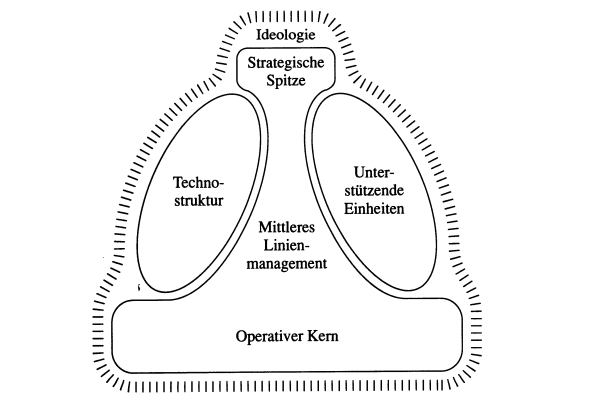
\includegraphics[scale=0.6]{basic_types.png}
\caption{Basic types of organizations. \cite[p. 110]{Mintzberg}}
\label{fig:basic_types}
\end{figure}

\subsection{Coordination Mechanisms}

Coordination mechanisms amount to six different types (illustrated in Figure~2
in Appendix). Mutual agreement is an informal agreement between employees --
the operators. Direct control is carried out by the strategic top and passed
on to the operators. Standardization of the work process is passed on to the
operators by the technostructure in the form of agreements in order to achieve
consistency in the work processes. In contrast, the standardization of the
results is the consistency in the presentation of the work results. Then
standardization of skills establishes coordination in the form of training of
operators. Workers are thus aligned with each other. Last, alignment of
beliefs of the organization occurs through standardization of norms.

\subsection{Basic Types of Organisations}

The basic types of organizations are divided by Mintzberg into seven different
units (listed in Table~1). The \emph{entrepreneurial organization} is
characterized by a simple, informal and flexible structure, usually consisting
of a simple strategic top and the operators. The other components are not yet
developed in this configuration. The organizations usually start in this
structure and are surrounded by a simple but dynamic environment with a lot of
competition.  Certain leadership qualities such as authority and charisma are
prerequisites for leaders in this configuration. Even under crisis and change,
this configuration can occur, needing a visionary view and a rough roadmap
that keeps the organization alive. The company has a specific mission, which
also makes it vulnerable and carries risk. Most companies fail in this
configuration because the mission does not always match reality.

The \emph{machine organization} is characterized by permanence in its
configuration. Bureaucracy is its characteristic. The technostructure is
crucial because it is where the work processes for the entire organization are
established. The mode of operation is clocked and planned through. The
environment is stable and the configuration is usually found in larger,
established companies. Strict rules give the configuration its stability even
in changing conditions. Efficiency and reliability characterize the image of
the organization, but the fixation on control can cause the organization to
fail in upheavals.

The \emph{diversified organization} is characterized by different divisions
and tends more towards the aforementioned machine organization. An autonomous
management envelops the different divisions with their strategy. This form is
mostly found in different market segments and has already reached a kind of
maturity. It is increasingly found in governments or public sectors. As a
result, they tend to focus on economic rather than social goals. Divisions can
retain their individuality by pursuing their own strategies as long as they
fit the overall strategy. The organization can distribute risk through its
form and include or omit different strands of the business. The disadvantages
are that innovations can only be implemented very slowly and they can also act
in a socially irresponsible manner.

The \emph{organization of professionals} is bureaucratic but decentralized in
the form of various institutes, with control resting with the professionals.
The context of the organization is complex but stable. Strategies are mostly
heterogeneous. Decisions are made based on the judgment of the professionals
or collective decisions. The advantages of the democratic decision-making
process often also lead to coordination problems. Innovations cannot be
implemented quickly because the professionals rely on their knowledge and
cannot reorient themselves.

In contrast, the \emph{innovative organization} is very dynamic and organic
and is built by experts in multidisciplinary teams. Coordination is usually
through direct arrangements and the strategic top and the operators are not
clearly separated. These organizations are mostly young and focus on the
learning and growth process. The main goal is innovation, which comes at the
expense of efficiency. The goal is more important than economic profitability.
An external operational core may be brought in.

The \emph{missionary organization} is defined by its ideology. Differentiation
from other organizations is its unique selling point and is usually
accompanied by charismatic leadership. The configuration may overlap with
others, especially in entrepreneurial, innovative, or even machine
organizations or organizations of professionals.

The \emph{political organization} is characterized by conflict and can overlap
other configurations, but is capable of holding it own. Coordination is
usually present in the form of a power play, which leads to confrontation and
uncertainty. Change is necessary and comes to light through political action.

\begin{table}[ht]
  \begin{tabular}{|p{3cm}|p{3.8cm}|p{3.8cm}|p{3.8cm}|}\hline
    Configuration & Primary coordination mechanism & Key part of the
    organization & Type of dezentralization \\\hline\hline

    Entrepreneurial & Direct control & Strategic top & Vertical and horizontal
    centralization\\ \hline

    The machine organization & Standardization of work processes &
    Technostructure & Limited horizontal decentralization \\ \hline
    
    Professionals & Standardization of skills & Operational core & Horizontal
    decentralization\\ \hline

    Diversified & Standardization of outputs & Middle line management &
    Limited vertical decentralization\\ \hline

    Innovative organization & Mutual coordination & Supporting units &
    Selective decentralization\\ \hline

    Missionary organization & Standardization of standards & Ideology &
    Decentralization\\ \hline

    Political organization & None & None & Various\\ \hline
\end{tabular}
\caption{Basic types \cite[p. 120]{Mintzberg}}
\label{Tab:types}
\end{table}

\subsection{Fundamental Forces in Organisations}

According to Mintzberg, the configurations should be seen as an integrated
framework of fundamental forces (see Figure~3 in Appendix). Each force must be
connected to a counterforce to keep the organization alive. Entrepreneurial
organizations tend to have a direct force initiated by the leader. The machine
organization is usually characterized by efficiency. Professionals want to
expand their skill set and break free from control. Diversified organizations
tend to concentrate power. Innovative organizations want to bring about change
and adaptation through the learning process. An organization's
self-destruction is avoidable only by applying the principles of cooperation
and competition, with policies and ideological beliefs in opposition.

\subsection{Life Cycle Model of Organisations}

Mintzberg contextualizes the above configurations with their associated forces
in terms of a life cycle model (see Figure~4 in Appendix). Configurations are
divided into formation stage, development stage, maturity stage, and decline
stage. Transitions between configurations are initiated by political
confrontations or tend to revitalization, a renewal of the configuration. As
mentioned above, organizations mostly start in the form of entrepreneurial
organization in the formation stage. These organizations are characterized by
a mission and are maintained as long as the leader is in charge. The demise of
the organization due to the above reasons is symbolized by a tombstone in each
case. Self-correction is not present in this configuration.

The missionary organization is most likely as the following configuration,
because there the charisma of the leader is installed as beliefs. Further
following there are two possibilities for an advancement of the
entrepreneurial configuration, if it is based on expert knowledge: Either it
tends to the innovative configuration, when its mission shapes its progress
through creativity, or to the professional organization, where a
standardization of skills is preferred.

On the other hand, the entrepreneurial configuration can become a machine
configuration, divided into instrumental and closed machine. The instrumental
machine is created by the takeover of an external influencer or a power
takeover from outside the organization. When internal management is strong
enough to assert itself, the entrepreneurial organization transforms directly
into a closed machine organization. The transition from missionary
configuration to closed machine occurs through the ideologized inefficiency of
the organization. From instrumental to closed machine organization, the
transition is characterized by an adjustment of internal stability.

Starting from the closed machine organization, it then tends to diversify as
it expands in size and influence. Bureaucratic status is placed at a new level
and revitalization resembles a proliferation of individual divisions. With
little external control, the closed machine organizations and the professional
organization tend to become politicized, which can lead to moral decay.

In the innovative configuration, political processes are seen as a temporary
difficulty which can lead to a turnaround or revitalization. Lastly, the
political configuration usually leads to the demise of these if it lasts too
long, as organizations cannot sustain long periods of conflict.

\subsection{Control Mechanisms of Organisations}

In the context of the life cycle model, Mintzberg already highlights the
hypothesis that organizations are kept alive for too long, which could be
replaced by other organizations and would allow a more sensible, productive
use of free resources. He critiques this form of control through mechanisms
(see Figure~5 in Appendix) realized by government and economic policies. "We
create organizations so that they serve us. But somehow they also force us to
serve them." \cite[p. 307]{Mintzberg}.

Mintzberg distinguishes between eight different control mechanisms:
\emph{nationalization} here means government interference when a task is
recognized as important but not covered by the private sector. In addition,
nationalization is considered when an organization's tasks are so closely
related to state activities that it can be run as a "direct arm of the state."
\emph{Democratizing} is understood as facilitating the expansion of corporate
governance, with power being constitutionally decentralized. \emph{Regulating}
organizations occurs through obligations from regulators and courts to the
organization to perform certain activities. Limits can also be imposed on
them, leaving internal control with managers. \emph{Exerting pressure} is
meant as encouraging organizations to adjust their behavioral fundamentals.
For example, activist campaigns aim to make organizations act in a socially
responsible way. \emph{Trust} means that business leaders are trusted to
observe social goals on their own -- simply because it is a "good thing" to
do. The difference with \emph{ignoring} is that a strong economy is seen as a
prerequisite for achieving social goals. Economic goals cover social goals as
well.  \emph{Incentives} can be donated, mostly in the form of subsidies for
organizations. These receive rewards through constraints. \emph{Restoring} is
equating freedom through entrepreneurship, with economic profit as an
indicator of good behavior. Mintzberg notes that financial incentives do not
belong where a company has caused a problem, but has the ability to solve a
problem caused by others. One should not reward a company for acting "badly."

\subsection{Comparison of System Development}

Alexander Solodkin in his publication \emph{Discovery of key problem causes in
  organizations} \cite{solodkin} presents distortions and noise as the main
problems in organizations. Accordingly, problems are the gap between the
current and the desired state of the system. Therefore, both states should be
described as accurately as possible. This difference has already been
clarified in \cite{graebe:2021} in the evolution of systems over time. Here,
an additional distinction is made between the states and the transformations.
Starting from the present system, the system as demanded is achieved by a
desired transformation. The true transformation, which takes place in the
implementation, leads to the system, which actually arises. A contradiction
arises between the ideal and the real line of development. In the TRIZ concept
of the Ideal Final Result (IFR), according to Solodkin, the desired system
state can be described.

In Mintzberg's expositions of the configurations of organization, the aspired
system states and the actual system states are not distinguished. The
transitions between configurations are presented by Mintzberg as laws that are
passed through purely political processes. Since we are dealing with
socio-economic and cultural systems, respectively, according to Solodkin, the
processes are subject to various biases and noises that Mintzberg ignores in
his description of configurations and the life cycle model of organizations.
While Mintzberg cites various forces that influence the organization, these
all arise from within the organization itself. External influences such as the
capital market, ecological influences, or material do not find sufficient
description in Mintzberg's model.

The implementation form of an organization, which brings it to the next
configuration to expand or overcome obstacles, is not specified. The stages of
the organization seem to exist as givens by Mintzberg and are not given a
developmental dimension outside of political confrontations. The difference
between development of the system, development of the components of the system
(here: actors, managers, technostructure, etc.) and relationships within the
system is not put into context. Throughput, deliberate processes of change, or
activities by management are not included in the life cycle model.

Mintzberg's two main assumptions, first, that organizations exist as stable
and persistent forms, "but their status changes regularly"
\cite[p. 287]{Mintzberg} and second, that forms are always in different
"stages of life," i.e., the organization is in the stages of birth, growth,
maturity, and decline or death, describes the changes solely in the power
constellation of organizations. In contrast, structural change, which is
consciously or unconsciously shaped by management, is only present in
descriptive form and, according to Mintzberg, seems to be more or less subject
to chance. The problem analysis, which would make the transformations
predictable, contradicts Mintzberg's emergent strategy development and does
not find application in the life cycle model.

\section{Conclusion}

For a sufficient description of management structures and the associated
application scenarios in different organizational structures, Mintzberg's
theses are insufficient in an academic setting. A system theoretical approach,
which brings forth the context of an organization in description and
implementation level, can only be seen from the perspective of a subjective
transformation to "better management" through Mintzberg's presentation of
emergent strategy development. The analogies presented are not so much
presented as a scientific analysis of processes of management, but are
intended to highlight an individual view of the social organization itself.

Mintzberg aims to take a socially critical stance through an experiential
description of processes in everyday work that relies less on actual academic
inquiry and instead views the concentration of power through organizational
structures in society through the "eyes of the manager." In his models, he
does not so much expose a framework for action that looks at system processes
at their core, but ultimately criticizes the politicized basis for successful
management that he believes has "made society uncontrollable"
\cite[p. 331]{Mintzberg}. His accounts are therefore not to be seen as
sociotechnical investigations and are therefore unsuitable for the
institutionalized use and associated scholarly reflection mentioned at the
outset.

On a tactical, subjective level, Mintzberg's view may nevertheless be helpful,
or as he describes it in the preface to his book, "This book is written for
those who spend their public lives with organizations and recover from them in
their private lives."

\newpage

\begin{thebibliography}{Gra21b}

\bibitem[Ans91]{ansoff} \textsc{Ansoff}, H.~I.: \newblock Critique of Henry
  Mintzberg‘s \emph{The Design School: Reconsidering the Basic Premises of
  Strategic Management}.  \newblock {In: }\emph{Strategic Management Journal}
  12 (1991), pp. 449--461.

\bibitem[Bur54a]{burns} \textsc{Burns}, Stewart: \newblock \emph{The
  Directions of Activity and Communication in a Departmental Executive Group}.
  \newblock Human Relations, 1954.

\bibitem[Bur54b]{stewart2} \textsc{Burns}, Stewart: \newblock \emph{Managers
  and Their Jobs}.  \newblock Human Relations, 1954.

\bibitem[Dav57]{davis} \textsc{Davis}, Robert~T.: \newblock \emph{Performance
  and Development of Field Sales Managers}.  \newblock Cambridge: Division of
  Research, Harvard Business School, 1957.

\bibitem[Gra20]{graebe:2020} \textsc{Graebe}, Hans-Gert: \newblock Technical
  Systems and Their Purposes.  \newblock In: TRIZ-Anwendertag 2020 (Oliver
  Mayer, ed.), Springer Verlag 2021, S. 1-13. \newblock
  \url{http://dx.doi.org/10.1007/978-3-662-63073-01}.

\bibitem[Gra21a]{graebe:2021} \textsc{Graebe}, Hans-Gert: \newblock On the
  concept of system in the Theory of Dynamical Systems.  \newblock (2021).
  \newblock
  \url{https://github.com/wumm-project/Seminar-S21/blob/master/Lecture/TDS.md}.
  
\bibitem[Gra21b]{seminar} \textsc{Graebe}, Hans-Gert: \newblock Seminar Notes:
  Summer Term 2021.  \newblock (2021).  \newblock
  \url{http://www.dorfwiki.org/wiki.cgi?HansGertGraebe/LeipzigerGespraeche/2021-07-23}

\bibitem[Jay]{Jaynes} \textsc{Jaynes}, Julian: \newblock Summary of Evidence
  for the Bicameral Mind Theory.  \newblock
  \url{https://www.julianjaynes.org/about/about-jaynes-theory/summary-of-evidence/'}

\bibitem[Min73]{Mintzberg2} \textsc{Mintzberg}, Henry: \newblock \emph{The
  Nature of Managerial Work}.  \newblock New York: Harper \& Row, 1973.

\bibitem[Min91]{Mintzberg} \textsc{Mintzberg}, Henry: \newblock
  \emph{Mintzberg über Management}.  \newblock Gabler Verlag, 1991.

\bibitem[Que56]{guest} \textsc{Quest}, Robert~H.: \newblock \emph{Of Time and
  the Foreman}.  \newblock Personnel, 1956.

\bibitem[Shp]{shpakovsky} \textsc{Shpakovsky}, Nikolay: \newblock Human and 
  technical systems.  Online, 2003. \newblock
  \url{https://wumm-project.github.io/Texts/Shpakovsky/mts-ru.pdf}

\bibitem[Sol]{solodkin} \textsc{Solodkin}, Alexander: \newblock Discovery of
  Key Problem Causes in Organisations.  Online, 2020.\newblock
  \url{https://wumm-project.github.io/Texts/Solodkin-TDS2020-en.pdf}

\bibitem[Ste51]{stewart} \textsc{Stewart}, Rosemary: \newblock \emph{Managers
  and their Jobs}.  \newblock New York: McMillan, 1951

\end{thebibliography}

\clearpage

\section{Appendix}

\begin{center}
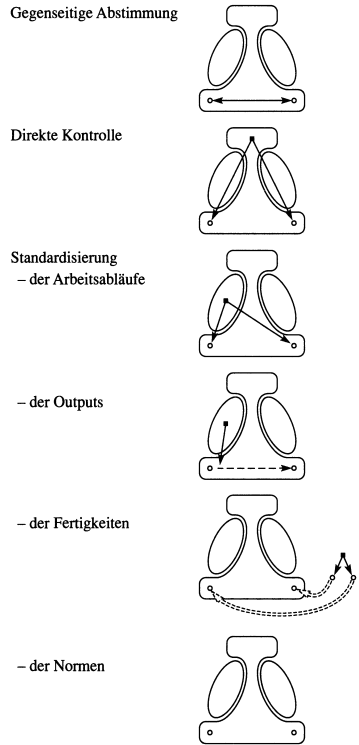
\includegraphics[scale=0.7]{koordinationsmechanismen.png}\\
{Coordination mechanisms: Mintzberg on Management, Henry Mintzberg:
  1991 p.113}
\label{fig:coordination}

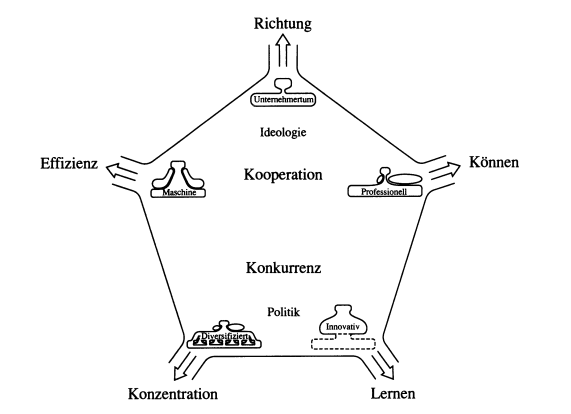
\includegraphics[scale=0.7]{forces.png}\\
{Coordination mechanisms: Mintzberg on Management, Henry Mintzberg:
  1991 p.264}
\label{fig:forces}

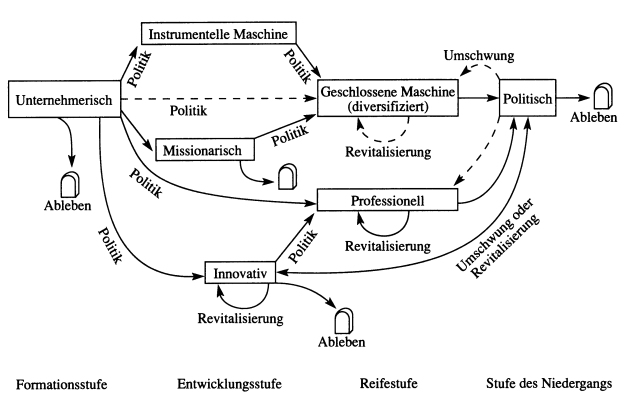
\includegraphics[scale=0.7]{lifecycle.png}\\
{Life cycle model: Mintzberg on Management, Henry Mintzberg: 1991
  p.288}
\label{fig:lifecycle}

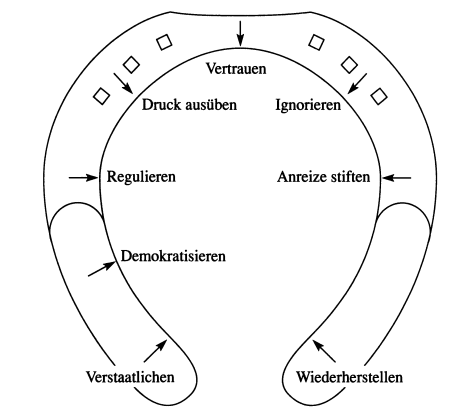
\includegraphics[scale=0.7]{control.png}\\
{The conceptual horseshoe: Mintzberg on Management, Henry Mintzberg:
  1991 p.312}
\label{fig:control}
\end{center}
\end{document}
